\documentclass[a4paper]{article}
\usepackage[utf8]{inputenc}
\usepackage{amsmath, amssymb}
\usepackage{fancyhdr}
\usepackage{ amssymb }
\usepackage{tikz}
\usepackage{pgfplots}


\pagestyle{fancy}
\fancyhead[LO]{\small{2015 - machine learning project - paper} \\ \small{Michael Segert (J114030912), Alex Peyrard, Yajing Chen,
Haosheng Zhang, Jiachao Chen, Chunhui Ding}    }
\fancyhead[RO]{}
\fancyfoot[CO]{\thepage/5}
\setlength{\tabcolsep}{2pt}

\begin{document}


\section{Introduction }


\section{Project}
In this report, we illustrate how we manage to finish the group project of our machine learning course, which is to make Mario win the game in a fastest way without human intervention. After doing some research work on the Internet, we find two possible machine-learning related solutions to our task. One of them is to train a neural network with the help of genetic algorithms, while the other one is to use q-learning. Due to time limitation, we only implement the neural network one. But we still make a brief introduction to the q-learning method in this report.

\section{Background knowledge}
Since the approach introduced in this paper based on genetic algorithm and neural networks, this chapter presents an overview of both topics.

\subsection{Genetic Algorithm}
Genetic algorithm is a search heuristic that mimics the process of natural selection called evolution. It is used to solve optimizing and search problems. The main idea is generating generations of possible solutions until a certain quality of solution is archived. Every generation depends on the generation before. Every genetic algorithm based on the same following components: representation, selection, genetic operators and fitness function.
The representation deals with how to represent a solution for the given problem. Since genetic algorithm are supposed to solve optimization problems, the problems to optimize has to be represented in a proper way. This representation can be considered as DNA or gene model.
The selection determines what solutions get into the next generation. On a more precise scale, it regulates what solutions are allowed to insert their genes into the next generation throw solution pairing processed by genetic operators.
The genetic operators are used to generate solutions for a new generation. Mutation and crossover are two ways to achieve that. Mutation modifies genes according to a given probability with a random value. Crossover recombine the genes of two solutions together two one new one.
Finally the fitness function assesses all the solutions and allows comparing them to each other. The fitness of one solution shows the quality of it. The higher the quality, the better the solution.
A deeper look into the topic genetic generations shows~\cite{Jain96}.

\subsection{Neural Network}
Neural network is a technology to create an artificial intelligence inspired by biological neural network called brain. It based on several layers of nodes. The layers are connected to each other. Input and output layer represent the interface to the environment. The connections between the layers have weights to tune the signals. Those weights are used in the algorithm this paper presents. A deeper look into the topic neural networks shows.~\cite{Whitley93agenetic}.


\section{Image Recognition}
The image recognition is used to extract more information out of the given screenshot. That information enriches the input of our algorithm. On a more precise scale, the recognition finds the positions of all gaps and tubes, since those information are not provided by the interface itself. Additionally, positions of hovering boxes and rockets on the ground could be extracted as well. However, recognizing four different objects slows down the algorithm and doesn’t increase the solution quality.

\section{Algorithm}
The algorithm is subdivided into two parts: neural network and genetic algorithm.
The two parts work together to solve the problem mentioned before. The neural network controls the Mario counter in the game with the available commands in the game. Those commands are jump, run, go left and go right. Controlling the counter, the neural network is supposed to make Mario reach the finish as fast as possible.
The genetic algorithm is used to find a neural network what makes Mario reach the finish fast.


\subsection{Neural Network}
\label{subsec:neural}
The neural network is basically the player of the game and has the same input and output to interact with the game. It contains one input, one hidden and one output layer.
The input layer has 5 nodes what cover the following input sensors: Mario his distances to the closest enemy, the closest gap, the closest pipe. Also, the time since Mario his last jump and whether Mario stands on the ground or not. The hidden layer contains 10 nodes. The output layer produces 4 outputs and has 4 nodes. The outputs cover the buttons available in the game Super Mario:  Jump, run, go left and go right. Those buttons are triggered, when the output value of the belonging node passes 0.5. Additionally, every edge between two nodes has a weight.


\subsection{Genetic Algorithm}
The genetic algorithm contains settings such as selection, inheritance and fitness function. Those parts are introduced after an overview of the gene model and the initial population
The gene model represents one solution for the given problem. That means one solution contains all weight to configure the neural network structure introduced in chapter ~\ref{subsec:neural}. Furthermore one gene is one weight.
The population of every generation is fixed at the amount of 100 solutions. Furthermore the initialize population also called generation 0 is contains solutions with randomly generated gens.
Finally , the genetic aglorithm runs until a given number of generation has been processed.

\begin{itemize}

\item{Selection Strategy}
The algorithm uses an elite strategy. This strategy copies the first 3 fittest solutions into the next generation that allows keeping the best solution for sure. The remaining solutions will take part in a lottery to find partners for the heredity process. The chance to get selected in the lottery depends on the fitness of the solution. The better the fitness, the more likely to be selected for heredity. The lottery lasts until the next generation contains the maximum amount of 100 new solutions.


\item{Inheritance process - genetic operators}
The algorithm uses both genetic operators: mutation and crossover.

The mutation operator is applied to each gene of all Solutions. According to the mutation probability of (ASK), a random value between -1 and 1 is added to the gene value.

The crossover operator is applied to a pair of solutions. During this process, the values of both solutions for the same neural network weight compete against each other in a lottery. In this lottery both values have the same probability to get into the new solution for the new generation.

\item{fitness function}
The fitness function measured the fitness of a solution. It is related to the first level of the super Mario game. The solution is applied to the first level of super Mario. It controls Mario until he dies, reached the finish line or got stuck. Getting stuck is indicated by fitness function. If the fitness function doesn’t increase for some frames, Mario would be stuck. The fitness depends on two facts. First one is the distance between start of the level and current position of Mario. Second one is the remaining time after reaching the finish of the level. After reaching the finish, the remaining time is multiplied by 1000 and added to the path length from start to finish. Therefore a huge bonus is implemented for reaching the finish line. The further Mario went and the faster he reached the finish line, the higher is the fitness of the solution.

\end{itemize}



\section{alternative approach}

This chapter introduces brielfy a second way to solve the given problem aside our approach. It uses the Q-learning technique. \\ \\
Q-learning is a reinforcement learning algorithm. It works by learning the function Q(s,a), where s and a stands for states and actions respectively. The final values of Q(s,a) determines the action-selection policy in every state. In order to train Q(s,a), we have to decide 3 things, i.e., s (states), a (actions) and r(rewards). The function Q(s,a) is updated by the formula:
\[Q(state, action) = R(state, action) + \gamma * Max[Q(next state, all actions)] \]
Where $\gamma$ is the discount factor that controls the amount of influence that the future action have on the current state, R(state, action) is the reward function with respect to states and actions. We can design s, a, r depending on our project to make the algorithm work.


\section{Evaluation}
This chapter assesses our approach throw monitoring during the runtime. After showing the best solution for the first level of super Mario, a statistic about all generations is presented.

\subsection{Solution for Super Mario Game}
The algorithm was tested on an i7 Intel CPU with three running cores. It took 30 minutes to find a solution. This solution makes Mario reach the finish of the first level after 20,33 seconds.

\subsection{Statistics}
During the runtime, the fitness of every solution in every generation was tracked and all the data collected afterwards. The collected data are subdivided into best, worth and average solution of each generation and show the variance of the fitness during runtime in fig1. Furthermore, the average is differed into with and without elitism.

\begin{figure}[ht]
\centering
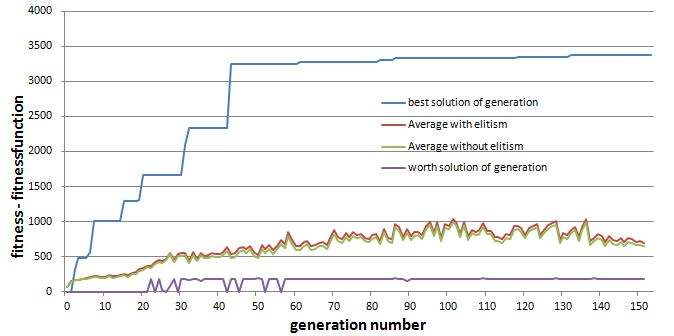
\includegraphics[scale=0.7]{statistic.jpg}
\caption{ statistics about generation fitness }
\label{fig1}
\end{figure}


The fig1 shows three facts. The first fact is after the 43th generation the peak of the fitness value is almost reached and all generations after the 43th generate only a small advantage. Second fact, both averages are cloth to each other, but don’t grow as strong as the best solution. Third fact, the worth solution is after one growing step constant. However, the worth solution of each generation doesn’t improve.

\section{Conclusion}
This work presented a reinforcement learning algorithm to learn how to finish the first level of the Super Mario game as fast as possible. On a more precise scale, a genetic algorithm and a neural network was introduced. Both parts are used to control Mario during the first level. The game runs in an emulator and offers an interface throw a systempipe. The genetic algorithm finds the fittest neural network. The neural network controls Mario in the game.  \\
This approach results a solution for that problem very fast. As shown in the evaluation, the quality or fitness of the neural network increases with runtime and processed generation. However, close to the peak of fitness or quality it converges very slowly. That means a solution can be found very fast, but on the other hand finding the perfect solution takes time. \\
In Conclusion, using a neural network in combination with genetic algorithm is not only fast in computing, but also fast in developing, since it doesn’t contain much high complicated mathematic. The main idea is to try and test neural networks in a guided and efficient way genetic algorithm provides.



\bibliography{lit}
\bibliographystyle{plain}


\end{document}

